\section{Arquitectura del entorno docente}
\subsection{Separar contenido, entorno y ejecución}
La arquitectura distingue tres capas. La primera contiene el problema científico: datos de ejemplo, ejercicios, explicaciones y criterios de interpretación. La segunda define el software necesario para trabajar. La tercera ejecuta comprobaciones y produce salidas. Esta separación permite modificar una pregunta sin rediseñar el entorno, o actualizar una dependencia sin reescribir toda la actividad.

Los contenedores de desarrollo describen un entorno mediante archivos versionados; GitHub Codespaces puede utilizarlos para ofrecer un espacio accesible desde el navegador \cite{devcontainers}. Esta descripción debe incluir dependencias y comandos de preparación. El acceso web reduce la necesidad de instalar herramientas científicas en cada equipo, pero sigue requiriendo una cuenta, conectividad y recursos disponibles. Un entorno descrito no es necesariamente inmutable: imágenes etiquetadas y paquetes sin fijar pueden cambiar entre ejecuciones.

Los repositorios docentes citados en el resumen incluyen \texttt{jupyter-on-codespaces} y\linebreak \texttt{exercises-silafae} \cite{repos}. La arquitectura que se presenta aquí sirve para documentar ese enfoque y su evolución. Antes de una evaluación formal, deben registrarse los commits exactos usados en cada escuela y las configuraciones efectivamente desplegadas. Consultar el estado actual de un repositorio no reconstruye automáticamente el entorno de una sesión histórica.

\subsection{Git y automatización como herramientas de razonamiento}
Git registra cambios en los materiales y permite relacionar una decisión con una revisión concreta. En una actividad de física, un cambio puede afectar la selección de eventos, una normalización o una figura. El estudiante debería poder explicar qué modificó y por qué, además de obtener una salida. El historial ayuda a revisar esas decisiones, aunque no sustituye la explicación científica.

La automatización ejecuta tareas previamente definidas. Un flujo puede comprobar que un cuaderno corre desde un estado limpio o generar una figura con parámetros conocidos. El resumen aceptado menciona GitHub Actions, GitLab CI/CD y una tarea denominada ``Process ATLAS ROOT Open Data'' \cite{abstract}. Esa descripción no demuestra paridad funcional entre todas las plataformas. La parte portable es el procedimiento cuando sus dependencias e interfaces están documentadas; la configuración del servicio de integración continua requiere adaptación y pruebas.

\begin{figure}[htbp]\centering
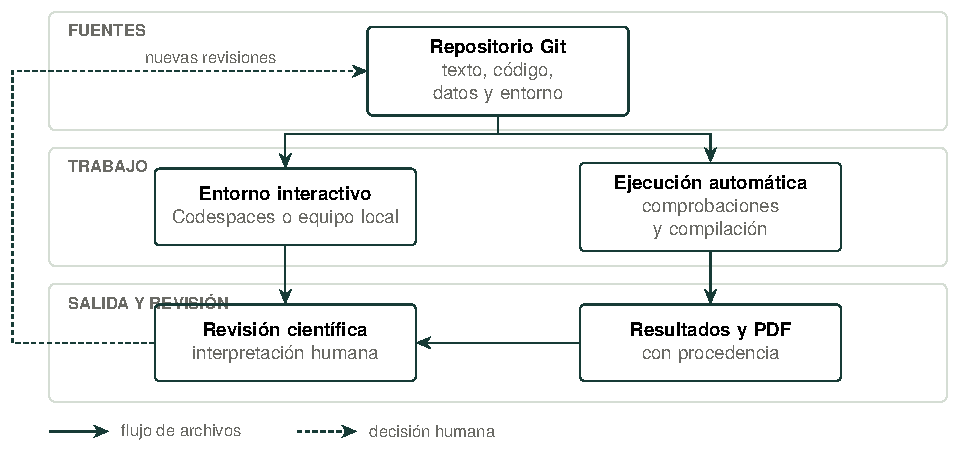
\includegraphics[width=160mm]{figures/modelo.pdf}
\caption{Arquitectura de referencia del trabajo docente y del demostrador editorial. El entorno interactivo y la ejecución automática consumen fuentes compartidas; la revisión científica sigue siendo una tarea humana.}\label{fig:arquitectura}
\end{figure}

\subsection{Una práctica de física que se pueda inspeccionar}
Como diseño docente proponemos partir de una distribución física sencilla producida a partir de datos abiertos. Una secuencia puede pedir reproducir la distribución de referencia, variar una selección, comparar el resultado y justificar la diferencia. Deben declararse unidades, muestra utilizada y normalización. Una comprobación automática puede detectar una columna ausente o una ejecución incompleta; no puede establecer por sí sola si una elección física es apropiada.

Conviene conservar una muestra pequeña para comprobar el funcionamiento y separar esa prueba del análisis completo. También debe evitarse que un cuaderno conserve resultados de una ejecución anterior incompatibles con su código actual. Ejecutarlo desde un estado limpio ayuda a detectar dependencias implícitas. Esta secuencia se propone como patrón de actividad; no se presenta como un nuevo resultado experimental ni se incluyen datos sintéticos que simulen una medición real.
